\section{Конфигурация}
\label{sec:Chapter3} \index{Chapter3}

\begin{figure}
    \centering
    Real \\
    
\includegraphics[scale=0.45]{./images/data/Real.jpg} \\
    Synthetic
    \\
    
\includegraphics[scale=3]{./images/data/Synthetic.jpg} \\
    SynForms
    \\
    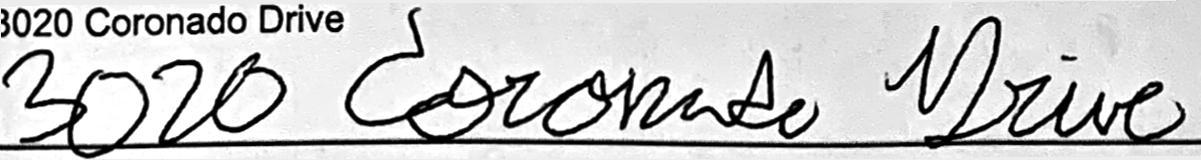
\includegraphics[scale=0.4]{./images/data/SynForms.jpg}
    \caption{\protect\hypertarget{image11}{Примеры изображений из датасета.}}
\end{figure}

\subsection{Описание модели}
В качестве энкодера использовался TransformerEncoder с следующими параметрами:
\begin{enumerate}
\item количество слоев: $6$
\item nhead в multiheadattention): $4$
\item размерномть feedforward сети: $768$
\item размерность пространства признаков: $128$
\end{enumerate}

В качестве сверточной нейронной сети для извлечения визуальных признаков использовался ResNet \hyperlink{cite.Kai15}{[17]}. В качестве функции активации использовалась ReLU. Далее архитектура ResNet описывается чуть подробнее:

\subsubsection{ConvBN}
Слой ConvBN представляет из себя композицию свертки (conv) и батч-нормализации (BN). Параметры BN следующие:
\begin{enumerate}
\item eps: $10^{-12}$
\item momentum: $0.01$
\end{enumerate}
За filters будем обозначать количество фильтров свертки. За kernel размер ядра, padding и stride также есть соответсвующие параметры свертки.

\subsubsection{ResNetBlock}
Этот residual блок предстваляет из себя композицию трех ConvBN (с размерами ядра: $[1, 3, 1]$, padding: $[0, 1, 0]$). Функция активации: ReLU (как было сказано ранее).

\subsubsection{FeatureBlock}
Это композиция нескольких ResNetBlock. Также для всех FeatureBlock, кроме последнего, после ResNetBlock-ов есть еще ConvBN слой (kernel: $3$, padding: $1$). В некоторых случаях (кроме последних двух) данный блок завершается max-pool (kernel: $2$). После FeatureBlock для регуляризации использовался dropout \hyperlink{cite.Sut14}{[12]} (с вероятностью $0.1$).

Первый FeatureBlock отличается от остальных: он представляет из себя композицию двух ConvBN (kernel: $[3, 3]$, padding: $[1, 1]$) и max-pool (kernel: $2$) слоя.

\paragraph{}

ResNet преставляет из себя композицию нескольких FeatureBlock-ов (всего $5$, с количествами ResNetBlock: $[1, 2, 5, 3]$, первый FeatureBlock отличается от остальных). После FeatureBlock-ов идут два ConvBN и dropout (c вероятностью $0.2$). 


\subsection{Описание датасета}

Данные можно разделить на три категории:
\begin{enumerate}
\item Real: Данные, собранные с документов. Обычно это поля различных контрактов, форм, или поля на счетах
\item SynForms: Написанные людьми строки текста
\item Synthetic: Псевдорукописные шрифты после применения некоторых аугментаций
\end{enumerate}
Примеры изображений можно найти на \hyperlink{image11}{[Рис 11.]}. Для обучения брались данные из всех трех групп в соотношении $1:1:1$.

\begin{figure}
    \centering
    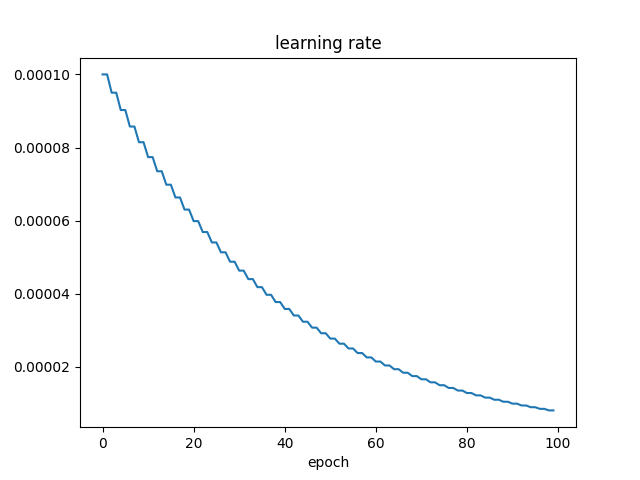
\includegraphics[scale=0.5]{./images/lr.png} 
    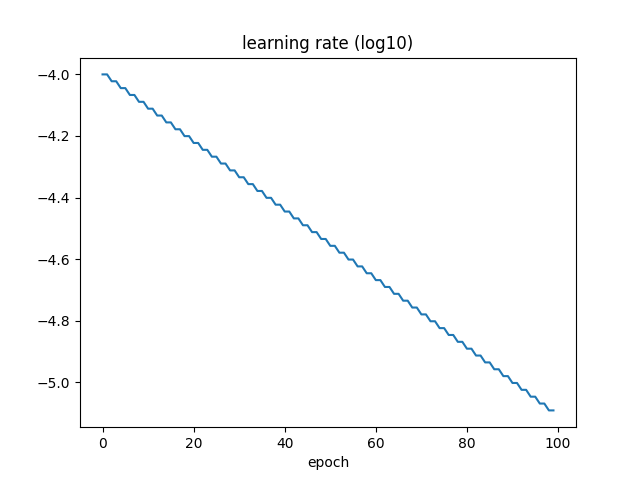
\includegraphics[scale=0.5]{./images/lr_log.png}
    \caption{\protect\hypertarget{image11}{Как менялся learning rate во время обучения.}}
\end{figure}

\subsection{Оптимизатор}
В качестве оптимизатора использовался AdamW \hyperlink{cite.Los17}{[29]} с параметрами:
\begin{enumerate}
\item betas: $(0.9, 0.999)$
\item weight decay: $0.01$
\end{enumerate}
Learning rate начинался с $0.0001$ и умножался на $0.95$ каждые две эпохи \hyperlink{image12}{[Рис 12.]}. Также во всех экспериментах размер батча был равен $64$. Использовалась точность \href{https://pytorch.org/blog/what-every-user-should-know-about-mixed-precision-training-in-pytorch/}{mixed precision в PyTorch}. Также, если не сказано иного, обучение ведется в течение $100$ эпох.

\subsection{Реализация mixup}
Для более эффективной работы, образцы $(x, y)$ и $(x_0, y_0)$ семплируются каждый раз внутри одного батча. Точнее говоря, если мы имеем батч $(x_1, \dots, x_N)$, то операция mixup выглядит следующим образом:

\begin{equation}
\begin{split}
y_{1:N} = shuffle(x_{1:N}) \\
\tilde{x}_{1:N} = \lambda x_{1:N} + (1 - \lambda) y_{1:N}
\end{split}
\end{equation}

Основываясь на результатах \hyperlink{cite.Bas19}{[16]}, по умолчанию (если не сказано иного) $\alpha = 0.5$, то есть $\lambda \sim Beta(0.5, 0.5)$.

\newpage